\section{Storage Element: Latches}
\label{sec:stor-ele-latch}

A storage element in a digital circuit can maintain a binary state indefinitely (as long as power is delivered to the circuit), until directed by an input signal to switch states.

\textit{Storage elements that operate with signal levels (rather than signal transitions) are referred to as latches; those controlled by a clock transition are flip-flops}. Latches are said to be \textit{level-sensitive devices}; flip-flops are \textit{edge-sensitive devices}. The two types of storage elements are related because \textit{latches are the basic circuits from which all flip-flops are constructed}.

\subsection{SR Latch}
\label{subsec:sr-latch}

The \textit{SR} latch is a circuit with two cross-coupled NOR gates or two cross-coupled NAND gates, and two inputs labeled \textit{S} for set, and \textit{R} for reset. The \textit{SR} latch constructed with two cross-coupled NOR gates is shown in Fig. 5.3. 
\begin{figure}[H]
  \centering
  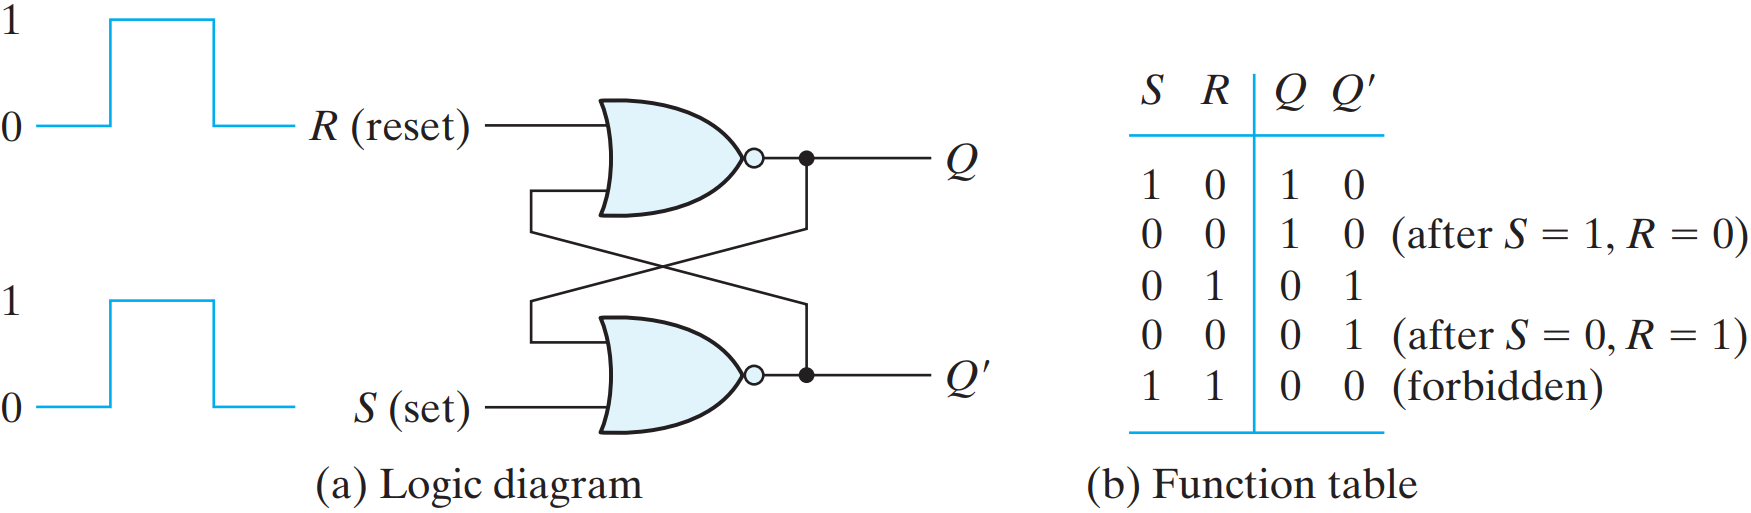
\includegraphics[width=\linewidth]{img/fig-5.3.png}
  \caption{SR latch with NOR gates}
  \label{fig:5.3}
\end{figure}
\noindent The latch has two useful states. When output $Q = 1$ and $Q' = 0$, the latch is said to be in the \textit{set} state. When $Q = 0$ and $Q' = 1$, it is in the \textit{reset} state.

However, when both inputs are equal to 1 at the same time, a condition in which both outputs are equal to 0 (rather than be mutually complementary) occurs. So, in pratice, \textbf{setting both inputs to 1 is forbidden}. Under normal conditions, both inputs of the latch remain at 0 unless the state has to be changed.

\vspace*{\fill}
\columnbreak

The \textit{SR} latch with two cross-coupled NAND gates is shown in Fig. 4. 
\begin{figure}[H]
  \centering
  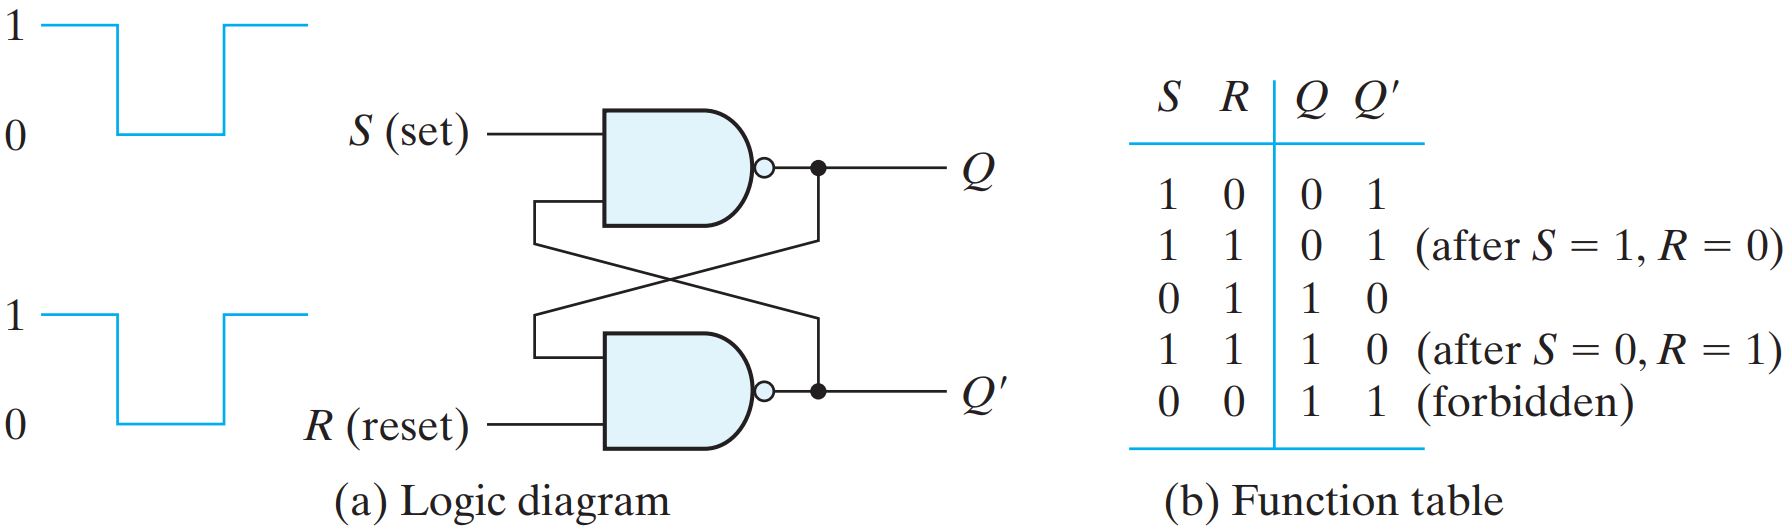
\includegraphics[width=\linewidth]{img/fig-5.4.png}
  \caption{SR latch with NAND gates}
  \label{fig:5.4}
\end{figure}
It operates with both inputs normally at 1, unless the state of the latch has to be changed. The condition that is forbidden for the NAND latch is both inputs being equal to 0 at the same time, an input combination that should be avoided.

The operation of the basic $SR$ latch can be modified by providing an additional input signal that determines (controls) when the state of the latch can be changed by determining whether $S$ and $R$ (or $S'$ and $R'$) can affect the circuit. An SR latch with a control input is shown in Fig. 5. It consists of the basic SR latch and two additional NAND gates.
\begin{figure}[H]
  \centering
  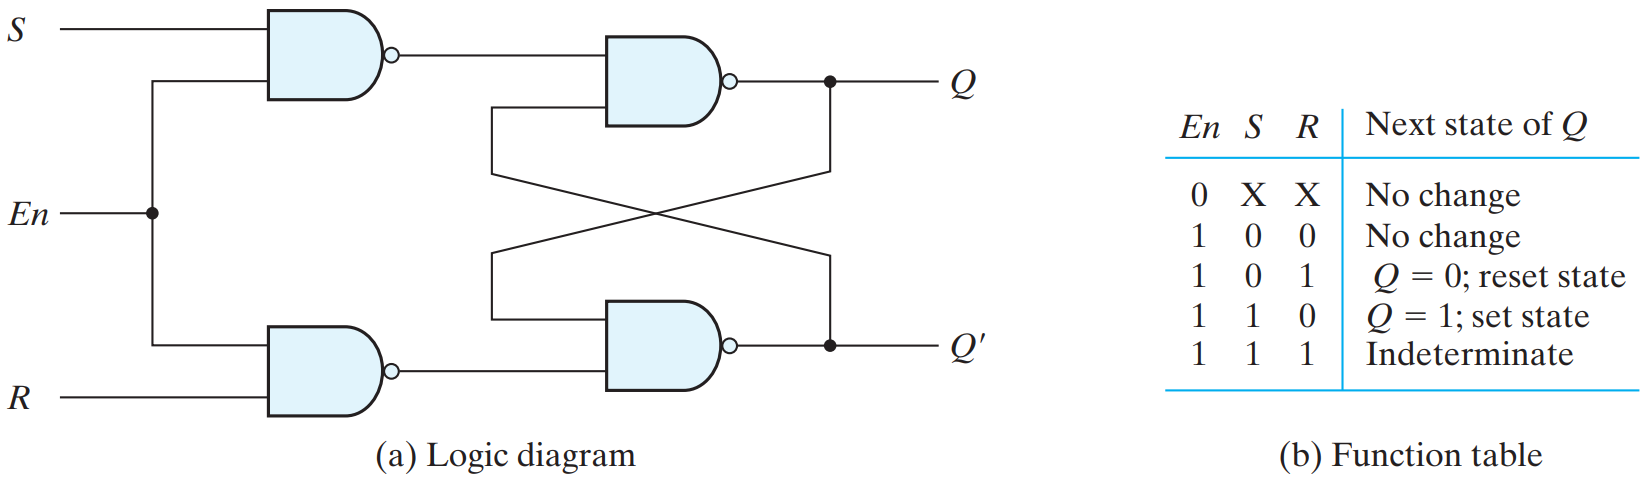
\includegraphics[width=\linewidth]{img/fig-5.5.png}
  \caption{SR latch with control input}
  \label{fig:5.5}
\end{figure}
An indeterminate condition occurs when all three inputs are equal to 1. This condition places 0's on both inputs of the basic $SR$ latch, which puts it in the undefined state.

\textbf{Note:}
\begin{itemize}[leftmargin=0.5cm]
  \item Input condition puts an $SR$ NOR latch into an indeterminate state is the condition ``Both inputs are 1''.
  \item Input condition puts an $SR$ NAND latch into an indeterminate state is the condition ``Both inputs are 0''.
\end{itemize}

\subsection{D Latch (Transparent Latch)}
\label{subsec:d-latch}

One way to eliminate the undesirable condition of the indeterminate state in the $SR$ latch is to ensure that inputs $S$ and $R$ are never equal to 1 at the same time. This is done in the $D$ latch, shown in Fig. 6. 
\begin{figure}[H]
  \centering
  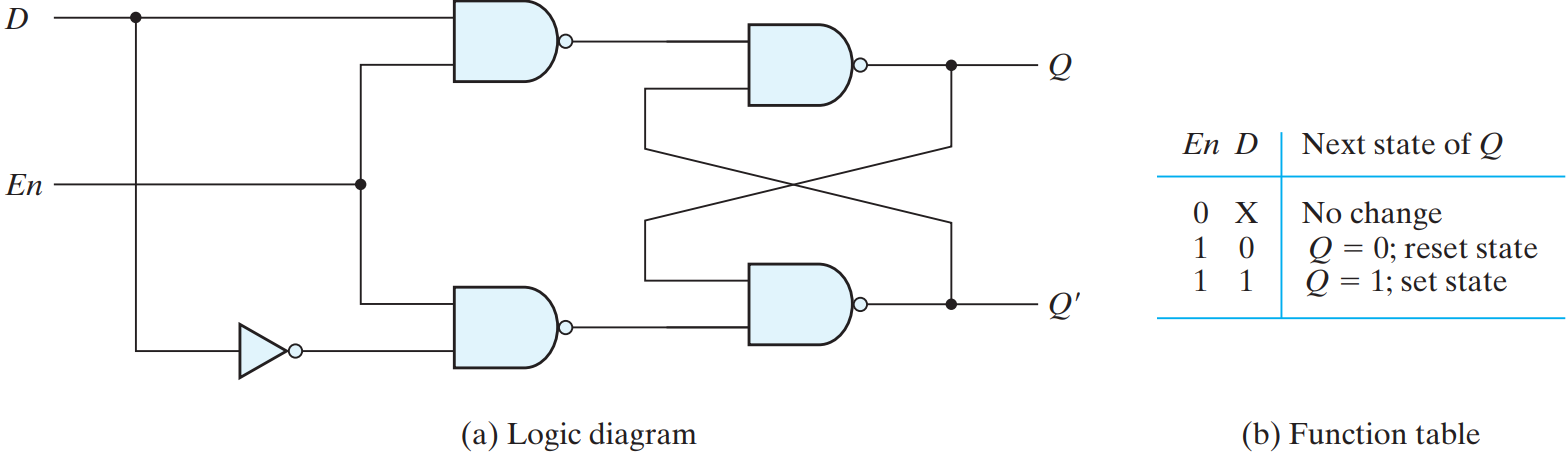
\includegraphics[width=\linewidth]{img/fig-5.6.png}
  \caption{D Latch}
  \label{fig:5.6}
\end{figure}
\noindent This latch has only two inputs: $D$ (data) and $En$ (enable). The $D$ input goes directly to the $S$ input, and its complement is applied to the $R$ input. 

The binary information present at the data input of the $D$ latch is transferred to the $Q$ output when the enable input is asserted. The output follows changes in the data input as long as the enable input is asserted.

The graphic symbols for the various latches are shown in Fig. 5.7.
\begin{figure}[H]
  \centering
  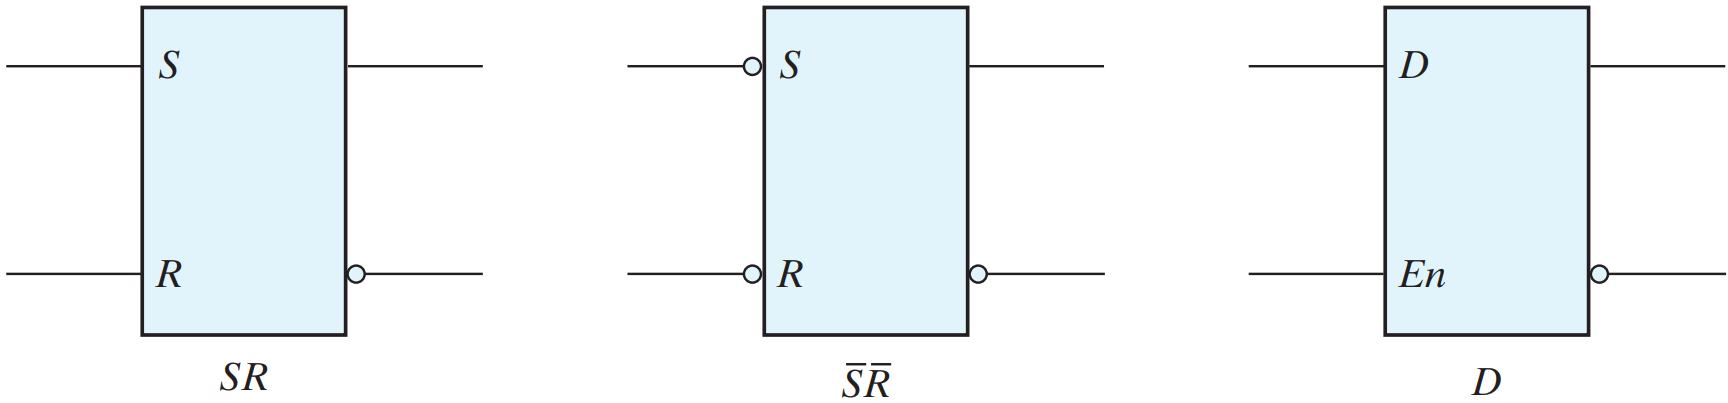
\includegraphics[width=\linewidth]{img/fig-5.7.png}
  \caption{Graphic symbols for latches}
  \label{fig:5.7}
\end{figure}

\textbf{Note:} A transparent latch has a data input, an enable input, and output. When the enable input is asserted, the output of the latch follows the input to the latch. When the enable input is de-asserted, the output of the latch is held at the value that was present at the moment the enable input was de-asserted.
